\chapter{\ifcpe ทฤษฎีที่เกี่ยวข้อง\else Background Knowledge and Theory\fi}

\section{ด้านการออกแบบ (Design)}
จากการศึกษาค้นคว้า พบว่าตัวโครงงานที่เรากำลังพัฒนามีการเปลี่ยนแปลงของ requirements อยู่บ่อยครั้ง เช่น สัปดาห์ก่อนลูกค้าต้องการให้แค่เช็คชื่อในวันปัจจุบันได้เท่านั้น  แต่พอสัปดาห์นี้ลูกค้าต้องการเช็คชื่อย้อนหลังด้วย
ทางผู้พัฒนาจึงจะนำแนวคิด design patterns \cite{designPatterns} เข้ามาช่วยในการทำงาน เนื่องจากแนวคิดนี้สามารถช่วยในการจัดการกับ requirements ที่มีการเปลี่ยนอยู่บ่อยครั้ง ให้มีความยืดหยุ่นมากขึ้น


หลักการ design patterns คือ แนวคิดที่ใช้ในการแก้ไขปัญหาที่มักเกิดขึ้นอยู่บ่อยครั้ง เช่น ในการออกแบบ software โดยแนวคิดเหล่านี้ไม่เป็นรูปแบบที่ตายตัว แต่เป็นการอธิบายผ่านแนวคิดหรือโครงสร้างที่จะถูกนำไปประยุกต์ใช้ตามสถานการณ์ต่างๆ  
โดยผู้พัฒนาได้นำแนวคิด agile \cite{agile}  ซึ่งเป็นแนวคิดจาก design patterns เข้ามาประยุกต์ใช้กับตัวโครงงาน 


Agile คือกระบวนการทำงานที่มุ่งเน้นการสื่อสาร ลดขั้นตอนการทำกับเอกสารลง แล้วนำมาพัฒนาชิ้นงานให้เสร็จเร็วยิ่งขึ้น  ซึ่งตัว agile นี้มีความน่าสนใจในส่วนของกระบวนการในการทำงานที่มีความโดดเด่นในเรื่องของความยืดหยุ่น  เนื่องจากวิธีดังกล่าวนี้มีการแจกแจงงานออกเป็นส่วนๆ  แล้วนำมาพัฒนากันเป็นทีละส่วน  
ซึ่งจุดเด่นของ agile นี้คือ การรองรับการเปลี่ยนแปลงของ requirements ซึ่งตอบโจทย์กับปัญหาการเปลี่ยนแปลง requirements ที่พบเจอ ทำให้ทางผู้พัฒนาสามารถส่งงานหรือตัว demo ให้กับลูกค้า และสามารถรับ feedback จากลูกค้ามาแก้ไขได้ เพื่อทำให้ตัวชิ้นงานมีความสมบูรณ์ยิ่งขึ้น 
 จากประโยชน์ทั้งหมดที่กล่าวมาข้างต้น ทางผู้พัฒนาจึงเลือกใช้ agile ใน flow การทำงานต่างๆ โดยทางผู้พัฒนาจะนำกระบวนการทำงานแบบ scrum~\cite{srcum} ดังแสดงในรูปที่~\ref{fig:Scrum}) มาใช้ในการวางแผนการทำงาน 
%
\begin{figure}
  \begin{center}
    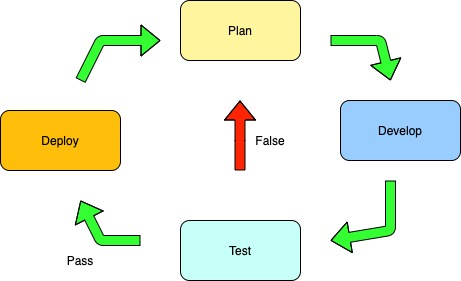
\includegraphics[width=\linewidth]{images/scrum.jpeg}
  \end{center}
  \caption[กระบวนการทำงานของ scrum]{กระบวนการทำงานของ scrum}
  \label{fig:Scrum}
\end{figure}
\CIreply{Fail instead of False?}


\CIreply{ซึ่งเจ้าตัว -- ทำไมชอบใช้คำว่า ``เจ้า'' จัง โหนเจ้าเหรอ}
Scrum เป็นหนึ่งในแนวคิดของ agile ซึ่งมีประสิทธิภาพในการจัดการกับปริมาณงานที่ได้รับให้มีความสมดุลเหมาะสม  โดยการแบ่งงานออกเป็นส่วนๆ แล้วแยกกันมาพัฒนา  ถ้าส่วนหนึ่งเสร็จแล้วจะมีการส่งไป test  หากผ่านขั้นตอนนี้จะเคลื่อนไปทำงานในส่วนถัดไป  หากไม่ผ่านก็จะวนกลับไปในขั้นตอนเดิมเพื่อกลับพัฒนาให้ดีขึ้นอีกครั้ง ซึ่งกระบวนที่กล่าวไปข้างต้นนี้  จะช่วยให้เราสามารถโฟกัสกับตัวชิ้นงานได้ดียิ่งขึ้น เนื่องจากมีการเจาะลงไปทำเป็นทีละส่วน ทำให้สามารถที่จะพัฒนาระบบได้อย่างมีประสิทธิภาพกว่าการทำเป็นชิ้นใหญ่เพียงครั้งเดียว


ในส่วนของการออกแบบฐานข้อมูล ทางผู้พัฒนาเลือกใช้ MongoDB \cite{MongoDB} ซึ่งฐานข้อมูลตัวนี้เป็นฐานข้อมูลแบบไม่มีความสัมพันธ์ (NoSQL) 
เหตุผลที่เลือกใช้ฐานข้อมูลตัวนี้เนื่องจาก MongoDB มี services และ tools หลายตัวที่ช่วยอำนวยความสะดวกในการจัดการกับข้อมูลเป็นอย่างดี เช่น MongoDB Atlas, MongoDB Compass 
ข้อดีอีกอย่างคือ NoSQL สามารถ scalable เพื่อรองรับการขยายฐานข้อมูลในอนาคต 

ในส่วนโครงสร้างของระบบทางผู้พัฒนาเลือกใช้แบบ client-server \cite{Client-Server} ส่วนการรับส่งข้อมูลใช้ RESTful API \cite{RESTFUL}
ในส่วนของการออกแบบ UX/UI ทางเราเลือกใช้เครื่องมือ Adobe XD \cite{AdobeXD} ซึ่งเป็น software ที่ใช้สำหรับวาดแบบหรือออกแบบหน้า UI เนื่องจากโปรแกรมนี้มีให้ใช้งานได้ฟรี และยังเรียนรู้และเริ่มต้นใช้งานได้ง่าย \CIreply{โดยไม่ต้องเสียเวลาไปเรียนรู้ -- ฟังดูขี้เกียจ}
  

\section{ด้านเทคนิค (Technical)}
ในส่วนของทฤษฎีหรือองค์ความรู้ในด้านนี้จะหนักไปในเรื่องของการทำ
web application ในส่วนของหน้าบ้าน (frontend) ทางผู้พัฒนาเลือกใช้ในตัวของ
React \cite{React} ซึ่งเป็น library ของ JavaScript ตัวหนึ่งที่ได้รับความนิยมเป็นอย่างมาก เหตุผลที่เลือกใช้เนื่องจากตัว library React นี้ถูกสร้างจากทาง Facebook 
จึงมี community อย่างหนาแน่น  เมื่อพบเจอปัญหาที่ไม่สามารถแก้ไขด้วยตนเอง สามารถไปค้นหาจากแหล่ง community เหล่านี้ได้ ยกตัวอย่างเช่น StackOverflow 
ยิ่งไปกว่านั้น เหตุผลที่เลือกใช้ React ก็คือ Redux \cite{Redux} ซึ่งเป็นเครื่องมือที่อำนวยความสะดวกในเรื่องของการจัดการกับ states ต่างๆ  ภายใน project ให้สามารถเรียกใช้ states ต่างๆ ได้อย่างเป็นระบบระเบียบ นอกจากนี้ การใช้งาน React ยังมีรูปแบบการเขียน
ได้หลากหลายรูปแบบ อย่างเช่น class components, hooks ซึ่งเราสามารถเลือกใช้ได้ตามความเหมาะสมของงานเพื่อทำให้ชิ้นงานมีประสิทธิภาพสูงสุด


ส่วนหลังบ้าน (backend) ทางผู้พัฒนาเลือกใช้ Node.js \cite{NodeJs}
และ Express.js \cite{Express} ซึ่ง Node.js ใช้สำหรับรันตัว JavaScript ไว้ทำงานบนฝั่ง backend ส่วน Express.js คือ  framework บน Node.js 
ซึ่งตัว Express มี features ต่างๆ  ที่จะช่วยเขียนอำนวยความสะดวกในการเขียน services เช่น การทำ routing (เพื่อให้ client สามารถส่งข้อมูลไปยัง server ได้) การจัดการ request และ response เป็นต้น  ทำให้เราสามารถพัฒนาเว็บโดยใช้ Node.js ได้สะดวกสบายยิ่งขึ้น
เนื่องจากทางตัวโครงงานฝั่ง frontend เราก็ใช้ภาษา JavaScript แล้ว backend เราก็เลยเลือกใช้ Express.js  เนื่องจากทางผู้พัฒนาจะได้ไม่ต้องเสียเวลาไปศึกษาภาษาอื่นๆ เช่น .NET Framework, Java, Python 
ส่วนประโยชน์ของ Node.js ก็คือในเรื่องของความเร็ว performance และยังง่ายและประหยัดเวลาต่อการศึกษาเรียนรู้\CIreply{ทำให้ไม่เสียเวลาในการเรียนรู้มาก -- ฟังดูขี้เกียจมาก}


\section{\ifcpe%
ความรู้ตามหลักสูตรซึ่งถูกนำมาใช้หรือบูรณาการในโครงงาน
\else%
ISNE knowledge used, applied, or integrated in this project
\fi
}

ความรู้ตามหลักสูตรที่ถูกนำมาใช้ในโครงงานมีดังต่อไปนี้
\begin{itemize}
  \item ความรู้จากวิชา Computer Programming ช่วยทำให้เข้าใจการเขียนโค้ดพื้นฐานและสามารถนำไปประยุกต์ในการเขียนภาษาอื่นๆได้
  \item ความรู้จากวิชา Basic Computer Lab ช่วยทำให้เข้าใจพื้นฐานการเขียน web application เบื้องต้นและเข้าใจคำสั่งพื้นฐานในการเขียน Linux CLI
  \item ความรู้จากวิชา Database ช่วยทำให้เข้าใจการออกแบบฐานและรู้คำสั่ง query ข้อมูลพื้นฐาน
  \item ความรู้จากวิชา Software Engineering ช่วยทำให้เข้าใจวงจรการทำงานให้เกิดเป็น software ชิ้นหนึ่งและเข้าใจว่ากระบวนการหรือแนวคิดในการสร้าง software มีอยู่หลากหลายวิธี สามารถเลือกใช้ได้ตามความเหมาะสมของชิ้นงาน 
  
\end{itemize}


\section{\ifcpe%
ความรู้นอกหลักสูตรซึ่งถูกนำมาใช้หรือบูรณาการในโครงงาน
\else%
Extracurricular knowledge used, applied, or integrated in this project
\fi
}

ความรู้นอกหลักสูตรที่ถูกนำมาใช้ในโครงงานมีดังต่อไปนี้
\begin{itemize}
  \item ความรู้เรื่องการเขียน React นำมาเพื่อเขียนหน้า browser ให้ทาง user ใช้งาน
  \item ความรู้เรื่องการใช้ Redux นำมาเพื่อใช้ในการจัดการกับ states ต่างๆในโค้ดส่วน frontend
  \item ความรู้ในการนำ Express.js เข้ามาช่วยในการเขียน routing, จัดการ requestและresponse
\end{itemize}
